\documentclass[a5paper,oneside]{amsart}
\usepackage[scale={.9,.9}]{geometry}
\usepackage{mathrsfs}
\usepackage{dsfont}
\theoremstyle{plain}
\usepackage{graphicx}
\newtheorem{theorem}{Theorem}
\newtheorem{lemma}{Lemma}
\newtheorem{corollary}{Corollary}
\newtheorem{proposition}{Proposition}
\newtheorem{conjecture}{Conjecture}
\theoremstyle{definition}
\newtheorem{problema}{Problema}
\newtheorem{ejercicio}{Ejercicio}
\newtheorem*{definition}{Definition}
\newtheorem*{remark}{Remark}
\usepackage{listings}
\lstset{
language=R,
basicstyle=\scriptsize
\ttfamily,
commentstyle=\ttfamily\color{gray},
numbers=none,
numberstyle=\ttfamily\color{gray}\footnotesize,
stepnumber=1,
numbersep=5pt,
backgroundcolor=\color{white},
showspaces=false,
showstringspaces=false,
showtabs=false,
frame=none,
tabsize=4,
captionpos=b,
breaklines=true,
breakatwhitespace=false,
title=\lstname,
escapeinside={},
keywordstyle={},
morekeywords={}
}
\title[Problemas de Procesos I]{Problemas de Procesos Estoc\'asticos I\\ Semestre 2013-II\\ Posgrado en Ciencias Matem\'aticas\\ Universidad Nacional Aut\'onoma de M\'exico\\TAREA 5}
\author{Antonio Soriano Flores}
\address{}
\usepackage[colorlinks,citecolor=blue,urlcolor=blue]{hyperref}
\input{definitions.tex}
\usepackage[colorlinks,citecolor=blue,urlcolor=blue]{hyperref}
\begin{document}
\maketitle
\begin{problema}
Sea $N$ un proceso Poisson de par\'ametro $\lambda$ y sea $T_n$ el tiempo de su en\'esimo salto. 
\begin{enumerate}
\item Pruebe que condicionalmente a $T_2$, $T_1$ es uniforme en $[0,T_2]$.
\begin{proof}
Como estamos en un proceso Poisson $\lambda$ entonces sabemos que:
 $$T_1=S_1 \sim Exp(\lambda)$$ 
 $$T_2=S_1+S_2 \sim Gamma(2,\lambda)$$
 $$T_2-T_1  =S_2 \sim Exp(\lambda)$$
 Adem\'as  $(T_2-T_1) \bot T_1$. Entonces:
 $$
 f_{T_1,T_2-T_1}(u,v)=\lambda e^{-\lambda u}\lambda e^{-\lambda u}\mathds{1}_{\set{u>0,v>0}}=\lambda^2e^{-\lambda(u+v)}\mathds{1}_{\set{u>0,v>0}}
 $$
 Luego definiendo el cambio de variable $X=T_1, Y=T_2-T_1$ lo que implica que $T_1=X,T_2=Y-X$ (con jacabiano igual a 1)  tenemos que la conjunta de $T_1$ y  $T_2$ es de la forma:
 $$
  f_{T_1,T_2}(t_1,t_2)=\lambda^2e^{-\lambda(t_2)}\mathds{1}_{\set{0 \leq t_1 \leq t_2}}
 $$ 
 Luego calculamos la densidad condicional $f_{T_1|T_2}(t_1|t_2)$ 
 $$
 f_{T_1|T_2}(t_1|t_2)=\frac{f_{T_1,T_2}(t_1,t_2)}{f_{T_2}(t_2)}=\frac{\lambda^2e^{-\lambda(t_2)} \mathds{1}_{\set{0 \leq t_1 \leq t_2}}}{(\lambda t_2)e^{-\lambda t_2}\lambda\mathds{1}_{\set{0 \leq t_2}}}=\frac{1}{t_2}\mathds{1}_{\set{0 \leq t_1  \leq t_2}}
 $$
 Obtenemos ahora la distribuci\'on de $T_2|T_1$, usando las propiedades de esperanza condicional.
 $$
 F_{T1|T_2}(u)=\probac{T_1\leq u}{T_2}=\espc{\mathds{1}_{\set{T_1 \leq u}}}{T_2}=h(T_2)
 $$
 donde $h$ es una funci\'on definida por:
 $$
 h(x)=\int_{0}^{x}\mathds{1}_{\set{t_1 \leq u}} f_{T_1|T_2}(t_1|x) dt_1=\int_{0}^{u}\frac{1}{x}dt_1=\frac{u}{x}
 $$
 Por lo tanto la distribuci\'on de $T_2|T_1$ es
 $$
F_{T1|T_2}(u)=\frac{u}{T_2}
 $$
 De donde concluimos que $T1|T_2$ se distribuye uniforme $(0,T_2)$
 \end{proof} 
\item Pruebe que si $W_1$ y $W_2$  son  exponenciales de par\'ametro $\lambda$  independientes entre si y de una variable uniforme $U$, entonces $U\paren{W_1+W_2}$ es una variable aleatoria exponencial de par\'ametro $\lambda$. 
\begin{proof}
Como $W_1$ y $W_2$  son  exponenciales de par\'ametro $\lambda$  independientes entonces $S=W_1+W_2$ tiene distribuci\'on Gamma(2,$\lambda$) luego supondremos que $U$ tiene distribuci\'on uniforme(0,1) es decir que tiene por densidad a $$f_U(u)=\mathds{1}_{0\leq u \leq 1 }$$
Luego por independencia de $U$ con $W_1$ y $W_2$ sabemos que la conjunta es el producto de la marginales y por tanto usando el teorema fundamental del calculo:
$$
f_{U,S}(u,s)=(\lambda)^2s e^{-\lambda s}\mathds{1}_{0\leq u \leq 1}\mathds{1}_{0 \leq s}ds
$$
Definamos a la variable $Y=U(W_1+W_2)=US$ entonces el problema se reduce a encontrar la densidad  la  de Y.
$$
f_Y(y)=F'_Y(y)=\frac{\partial}{\partial y}\p(Y\leq y)=\frac{\partial}{\partial y}\p(US  \leq y)=\frac{\partial}{\partial y}\p(S  \leq \frac{y}{U})
$$
$$
=\int_0^{\infty}f_{U,S} (\frac{y}{s},s)\frac{1}{s}ds=\int_0^{\infty}\lambda^2e^{-\lambda s}\mathds{1}_{0 \leq {y} \leq s}\mathds{1}_{0 \leq s}ds=\int_y^{\infty}\lambda^2 e^{-\lambda s}ds
$$
Por lo tanto:
$$
f_Y(y)=\int_y^{\infty}\lambda^2 e^{-\lambda s}ds=\lambda(1-(1-e^{-\lambda y}))=\lambda e^{-\lambda y}
$$
Por lo tanto $Y$ tiene distribuci\'on exponencial de par\'ametro $\lambda$.  
\end{proof}
\item Conjeture c\'omo se  generaliza lo anterior con $T_n$ y $T_1$.
\begin{proof}
Se proceder\'a como en el inciso 1, primero obtendremos la densidad conjunta  de $T_1,\ldots T_n$ a partir del hecho de que $T_1, T_2-T_1, T_3-T_2,\ldots T_n-T_{n-1}$ son variables independientes e id\'enticamente distribuidas como Exponenciales de par\'ametro $\lambda$.
$$
f_{T_1, T_2-T_1,\ldots ,T_n-T_{n-1}}(u_1,\ldots, u_n)=\prod_{i=1}^{n}\lambda e^{-\lambda u_i}=\lambda^n e^{-\lambda \sum_{i=1}^{n}u_i}
$$
De donde nuevamente definiendo el cambio de variable\\ $X_1=T_1, X_2=T_2-T_1,\ldots , X_n=T_n-T_{n-1}$  (Jacobiano de la transformaci\'on igual a 1) obtenemos que:
$$
f_{T_1, T_2, \ldots ,T_n}(t_1,\ldots, t_n)=f_{T_1, T_2-T_1,\ldots ,T_n-T_{n-1}}(t_1,t_2-t_1,\ldots,t_n-t_{n-1})
$$
$$
=\lambda^n e^{-\lambda \sum_{i=1}^{n}t_i-t_{i-1}}=\lambda^n e^{-\lambda t_n}
$$
Donde en la anterior ecuaci\'on definimos $t_0=0$.  Adem\'as recordemos que $T_n=\sum_{i}^{n}S_i$ y como  $S_i$ son independientes  exponenciales de par\'ametro $\lambda$   se sigue que $T_n$ tiene densidad Gamma(n,$\lambda$). Por lo tanto
$$
f_{T_n}(t_n)=\frac{(\lambda t_n)^{n-1}e{-\lambda t_n} \lambda}{\Gamma(n)}=\frac{\lambda^n t_n^{n-1}e^{-\lambda t_n}}{(n-1)!}
$$
Luego entonces la densidad conjunta de $T_1,\ldots, T_{n-1}$ dado $T_n$ esta dada por:
$$
f_{T_1,\ldots ,T_{n-1}|T_n}(t_1,\ldots, t_{n-1}|t_n)=\frac{\lambda^n e^{-\lambda t_n}}{ \frac{\lambda^n t_n^{n-1}e^{-\lambda t_n}}{(n-1)!}}=\frac{(n-1)!}{t_n^{n-1}}
$$
Ahora, recordemos que la densidad de los estad\'isticos de orden de una muestra de tama\~no $n-1$  proveniente de una poblaci\'on con  densidad $f$ esta dada por:
$$
f_{Y_1\dots ,Y_{n-1}}(y_1,\ldots ,y_{n-1})=(n-1)!f_{Y_1}(y_1)\ldots f_{Y_{n-1}}(y_{n-1})\mathds{1}_{\set{y_1\leq y_2 \ldots \leq y_{n-1}}}
$$
Luego entonces si tenemos una muestra de tama\~no $n-1$ de una distribuci\'on uniforme$(0,t_n)$  tendr�amos que:
$$
f_{Y_1\dots ,Y_{n-1}}(y_1,\ldots ,y_{n-1})=\frac{(n-1)!}{t_n^{n-1}}
$$
Es decir tiene la misma densidad que  la  conjunta de $T_1,\ldots, T_{n-1}$ dado $T_n$. Por lo tanto concluimos que  $T_1,\ldots, T_{n-1}$ dado $T_n$ tiene la misma distribuci\'on  que la distribuci\'on conjunta de los estad\'isticos de orden de un muestra de tama\~no $n-1$ de una poblaci\'on uniforme $(0,t_n)$. Lo anterior nos indica entonces que $T_i$ dado $T_n$  con $0 < i < n$ tiene la misma distribuci\'on que el i-\'esimo estad\'istico de orden es decir:
$$
f_{T_i|T_n}(t_i |t_n)=i {n-1 \choose i}\paren{\frac{t_i}{t_n}}^{i-1}\paren{1-\frac{t_i}{t_n}}^{n-1-i}\frac{1}{t_n} \mathds{1}_{0\leq t_i \leq t_n}
$$

\end{proof}
\item Escriba dos programas en Octave que simulen al proceso de Poisson de par\'ametro $\lambda$ en el intervalo $[0,1]$. En uno utilizar\'a s\'olo variables exponenciales y en el otro puede utilizar una variable Poisson.
\end{enumerate}
\end{problema}
\begin{problema}
%Simulaci\'on de un proceso Poisson puntual... subordinador...
 Sea $\Xi$ una medida de Poisson aleatoria en $(0,\infty)\times (0,\infty)$ cuya medida de intensidad $\nu$ est\'a dada por $\imf{\nu}{ds,dx}=\indi{x>0}C/x^{1+\alpha}\, ds\,dx$. 
\begin{enumerate}
\item Determine los valores de $\alpha$ para los cuales $\int 1\wedge x\,\imf{\nu}{dx}<\infty$. 
 \end{enumerate}
 \begin{proof}
 Supondremos que $\imf{\nu}{ds,dx}=\indi{s<t}\indi{x>0}C/x^{1+\alpha}\, ds\, dx$  y por lo tanto:
 $$
 \int 1\wedge x\,\imf{\nu}{ds,dx}=\int_0^t\int_0^1 x C/x^{1+\alpha} \, dx \, ds + \int_0^t\int_1^\infty  C/x^{1+\alpha} \, dx \, ds
 $$
 Para que la integral sea finita necesitamos que las dos integrales anteriores sean finitas, entonces para la primer integral suponiendo $\alpha \neq  1$ tenemos:
 $$
 \int_0^1 x C/x^{1+\alpha} dx =\frac{C}{1-\alpha} - C\lim_{x \rightarrow 0}\frac{x^{-\alpha+1}}{1-\alpha}
 $$
 El limite anterior existe cuando $\alpha < 1$. Por otro lado analizando la otra  integral y suponiendo $\alpha \neq 0$: 
 $$
  \int_1^\infty  C/x^{1+\alpha} dx=\frac{C}{\alpha}-C\lim_{x \rightarrow \infty}\frac{x^{-\alpha}}{\alpha}
 $$
 El limite anterior existe cuando $\alpha > 0$. Finalmente juntando las \'ultimas dos desigualdades concluimos que  $\int 1\wedge x\,\imf{\nu}{dx} < \infty$ cuando $\alpha \in (0,1)$
 \end{proof}
Nos restringimos ahora a valores de $\alpha$ para los cuales la integral anterior sea finita. Sean $\imf{f_t}{s,x}=\indi{s\leq t}x$ y $X_t=\Xi f_t$. 
 \begin{enumerate}
 \item Determine los valores  de $\alpha$ para los cuales $X_t<\infty$ para toda $t\geq 0$ casi seguramente.
 \end{enumerate}
 \begin{proof}
 Utilizando la proposici\'on 4.6 de las notas , sabemos que  $X_t=\Xi f_t$ es la integral de $f_t$ respecto a la medida de poisson aleatoria $\Xi$. El inciso (2) de esta proposici\'on nos indica que la variable  $X_t=\Xi f_t$ es casi seguramente finita si  la integral $\int 1 \wedge f_t dv$ es finita, por lo anterior calcularemos la integral involucrada:
$$
 \int 1 \wedge f_t dv  = \int \int _{\re^{2+}}  1 \wedge   \indi{s\leq t}x \indi{x>0}C/x^{1+\alpha}\, ds\,dx
$$
 $$
 =\int_0^1\int_0^{\infty}\indi{s\leq t}xC/x^{1+\alpha}\, ds\,dx+ \int_1^\infty\int_0^{\infty}\indi{s\leq t}C/x^{1+\alpha}\, ds\,dx
 $$
  $$
 =\int_0^1\int_0^{t}xC/x^{1+\alpha}\, ds\,dx+ \int_1^\infty\int_0^{t}C/x^{1+\alpha}\, ds\,dx
 $$
 $$
 =Ct\paren{\int_0^1 \frac{1}{x^{\alpha}}dx+\int_1^{\infty}\frac{1}{x^{1+\alpha}}}
 $$
 Y nuevamente, para que estas integrales sean finitas necesitamos que $\alpha \in (0,1)$.  Luego, si $\alpha \in (0,1)$ 
 $$
  \int 1 \wedge f_t dv =Ct\paren{\frac{1}{1-\alpha}+\frac{1}{\alpha}}=\frac{Ct}{\alpha(1-\alpha)}
 $$
 \end{proof}
 Nos restringiremos a dichos valores de $\alpha$. 
 \begin{enumerate}
 \item Calcule $\esp{e^{-\lambda X_t}}$ y pruebe que $X_{t}$ tiene la misma distribuci\'on que $t^{1/\alpha}X_1$. 
 \begin{proof}
 Nuevamente, utilizaremos la proposici\'on 4.6 de la notas, el inciso (1) de esta proposici\'on  nos dice que :
 $$
 \esp{e^{-\Xi f}}=\exp\paren{-\int\paren{1-e^{-f}}d\nu}
$$
 En nuestro caso sabemos que $X_t=\Xi f_t$ por lo tanto:
 $$
  \esp{e^{-\lambda X_t}}=\exp\paren{-\int\paren{1-e^{-\lambda f_t}}d\nu}
 $$
 Por lo que nos centraremos en el calculo de la integral : $\int\paren{1-e^{-\lambda f_t}}d\nu$.
 $$
 \int\paren{1-e^{-\lambda f_t}}d\nu=\int_0^{\infty}\int_0^{\infty} \paren{1-e^{-\lambda f_t}}C/x^{1+\alpha}\, ds\,dx
 $$
 Sustituyendo la funci\'on $\imf{f_t}{s,x}=\indi{s\leq t}x$ la integral se convierte en:
 $$
 =C\int_0^{\infty}\int_0^{t} \paren{1-e^{-\lambda x}}\frac{1}{x^{1+\alpha}}\, ds\,dx=Ct\int_0^{\infty} \paren{1-e^{-\lambda x}}\frac{1}{x^{1+\alpha}}\,dx
 $$
Para resolver esta integral recordemos que la distribuci\'on de una densidad exponencial de par\'ametro $\lambda$ es:
$$
F_X(x)=\int_0^{x}\lambda e^{-\lambda y}dy=1-e^{\lambda x}
$$
Entonces la integral buscada la podemos ver como sigue:
$$
Ct\int_0^{\infty} \paren{1-e^{-\lambda x}}\frac{1}{x^{1+\alpha}}\,dx=Ct\int_0^{\infty} \paren{\int_0^{x}\lambda e^{-\lambda y}dy}\frac{1}{x^{1+\alpha}}\,dx
$$
Haciendo cambio de orden de integraci\'on:
$$
=Ct\int_0^{\infty} \int_y^{\infty}\frac{\lambda e^{-\lambda y}}{x^{1+\alpha}}\,dx \,dy=Ct\int_0^{\infty} \lambda e^{-\lambda y} \paren{\int_y^{\infty}\frac{1}{x^{1+\alpha}}\,dx }\,dy
 $$
 Luego como suponemos que $\alpha \in (0,1)$ entonces $\int_y^{\infty}\frac{1}{x^{1+\alpha}}\,dx =\frac{y^{-\alpha}}{\alpha}$
 $$
=Ct\int_0^{\infty} \lambda e^{-\lambda y} \paren{\frac{y^{-\alpha}}{\alpha}}\,dy=\frac{Ct}{\alpha}\int_0^{\infty} \lambda e^{-\lambda y} y^{-\alpha}\,dy
 $$
 $$
 =\frac{Ct\lambda^{\alpha}}{\alpha}\int_0^{\infty}  e^{-\lambda y}(\lambda y)^{-\alpha} \lambda \,dy
 $$
 Recordando que la funci\'on Gamma;
 $$
 \Gamma(z+1)=\int_0^{\infty}t^ze^{-t}dt=\int_0^{\infty}(\lambda y)^ze{-\lambda y}\lambda\,dy
 $$
 Entonces:
 $$
 \frac{Ct\lambda^{\alpha}}{\alpha}\int_0^{\infty}  e^{-\lambda y}(\lambda y)^{-\alpha} \lambda \,dy= \frac{Ct\lambda^{\alpha}}{\alpha}\Gamma(1-\alpha)
 $$
 Por lo tanto:
\begin{equation}
   \esp{e^{-\lambda X_t}}=\exp\paren{-\frac{C\lambda^{\alpha}\Gamma(1-\alpha)t}{\alpha}}
\end{equation}
 Lo anterior nos esta dando la expresi\'on para  la funci\'on generadora de momentos de $X_t$ evaluada en $-\lambda$, entonces para verificar que $X_t$ tiene la misma distribuci\'on    que $t^{1/\alpha}X_1$  tenemos que ver que $   \esp{e^{-\lambda t^{1/\alpha}X_1}}= \esp{e^{-\lambda X_t}}$ para toda $\lambda$. Consideremos entonces la funci\'on $\phi(\lambda;t):=\esp{e^{-\lambda X_t}}=\exp\paren{-\frac{C\lambda^{\alpha}\Gamma(1-\alpha)t}{\alpha}}$. Como  lo anterior fue calculado para $t>0$ arbitrario entonces tomando $t=1$ obtenemos que:
 $$
 \phi(\lambda;1):=\esp{e^{-\lambda X_1}}=\exp\paren{-\frac{C\lambda^{\alpha}\Gamma(1-\alpha)(1)}{\alpha}}
 $$
Luego, evaluando la funci\'on en $\lambda t^{1/\alpha}$ obtenemos:
$$
 \phi(\lambda t^{1/\alpha} ;1):=\esp{e^{-\lambda t^{1/\alpha} X_1}}=\exp\paren{-\frac{C(\lambda t^{1/\alpha} )^{\alpha}\Gamma(1-\alpha)(1)}{\alpha}}
$$
Entonces:
$$
\esp{e^{-\lambda t^{1/\alpha} X_1}}=\exp\paren{-\frac{C\lambda^{\alpha}\Gamma(1-\alpha)t}{\alpha}}=   \esp{e^{-\lambda X_t}}
$$
 De donde se concluimos que  $X_t$ tiene la misma distribuci\'on    que $t^{1/\alpha}X_1$
  \end{proof}
 \item Diga por qu\'e el siguiente c\'odigo en Octave simula la trayectoria aproximada del proceso $X$ en el intervalo $[0,1]$.
\lstinputlisting{SuborEst.m}
 \end{enumerate}
 \begin{figure}
  \centering
    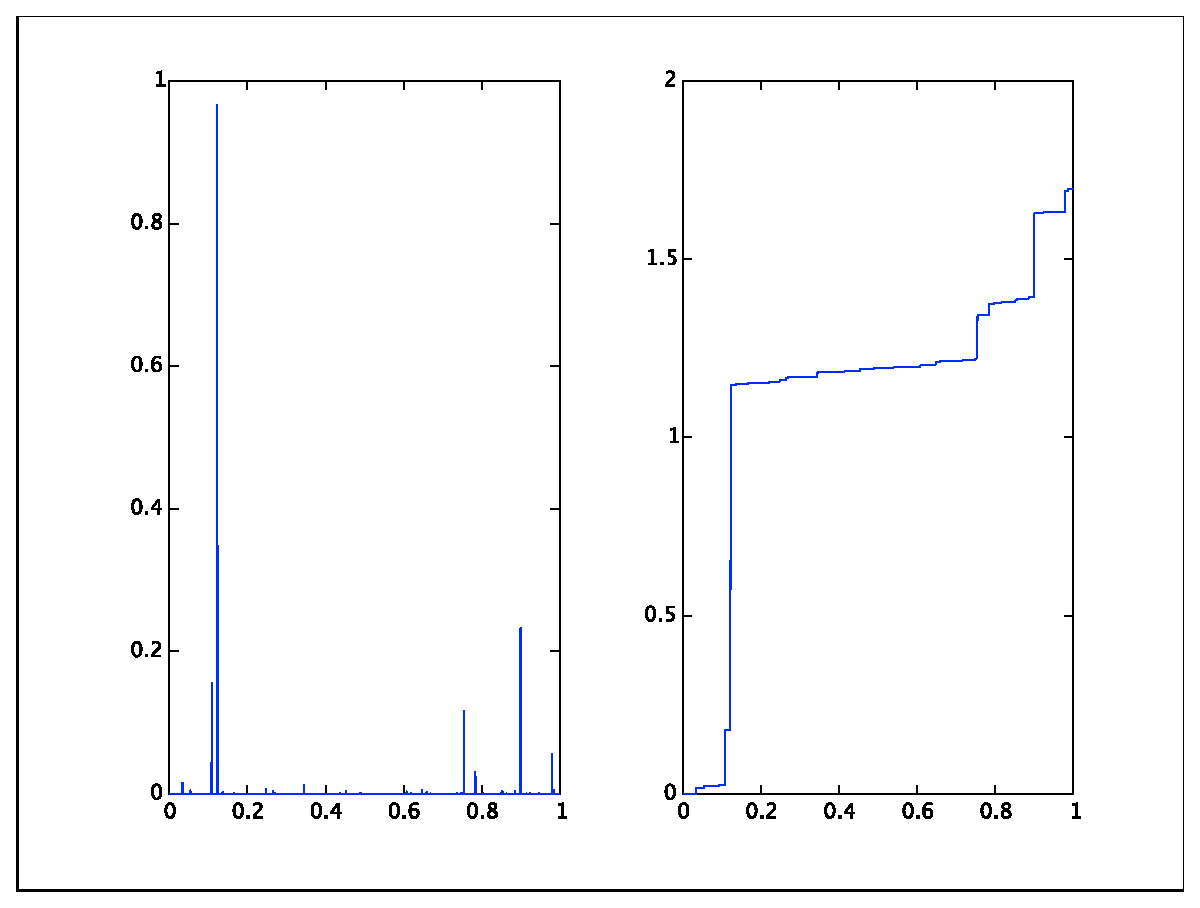
\includegraphics[width=0.7\textwidth]{Figure1.eps}
  \caption{Figura 1 Simulacion del proceso X}
  \label{fig:ejemplo}
\end{figure}

\end{problema}

\begin{problema}
Pruebe que si $X$ tiene incrementos independientes entonces el proceso $X^t$ dado por $X^t_s=X_{t+s}-X_t$ es independiente de $\F^X_t=\sag{X_s:s \leq t}$.
\begin{proof}
Sea $0 \leq s_1\leq s_2, \ldots ,\leq s_n$  y $0 \leq t_1\leq t_2, \ldots ,\leq t_m \leq t$  y definamos los eventos:
$$
A=\set{X_{t_1} \leq x_{t_1}, \ldots , X_{t_m} \leq x_{t_m}} \quad B=\set{X^t_{s_1} \leq x^t_{s_1}, \ldots , X^t_{s_n} \leq x^t_{s_n}}
$$
Notemos que $A \in \F^X_t$ y $B \in \sag{X^t_s: s \geq 0}$, demostraremos que $A$ y $B$ son eventos independientes.
$$
\p(A\cap B)=\p\paren{X_{t_1} \leq x_{t_1}, \ldots , X_{t_m} \leq x_{t_m},X^t_{s_1} \leq x^t_{s_1}, \ldots , X^t_{s_n} \leq x^t_{s_n}}
$$
$$
=\lim_{k \rightarrow \infty}\p\paren{X_{t_1} \leq x_{t_1}, \ldots , X_{t_m} \leq x_{t_m},X_t\leq k,X^t_{s_1} \leq x^t_{s_1}, \ldots , X^t_{s_n} \leq x^t_{s_n}}
$$
Recordando que $X^t_s=X_{t+s}-X_t$ lo que implica que $X^t_{s_2}-X^t_{s_1}=X_{t+s_2}-X_{t+s_1}$ entonces al construir incrementos independientes obtenemos:
$$
=\lim_{k \rightarrow \infty}\p\paren{X_{t_1} \leq x_{t_1},   \ldots ,X_t-X_{t_m} \leq k-x_{t_m},\ldots, X_{t+s_n}-X_{t+s_{n-1}} \leq x^t_{s_n}-x^t_{s_{n-1}}}
$$ 
Por la independencia en incrementos lo anterior es igual a:
$$
\p\paren{X_{t_1} \leq x_{t_1}, X_{t_2}-X_{t_1} \leq x_{t_2}-x_{t_1} ,\ldots ,X_{t_m}-X_{t_{m-1}} \leq x_{t_m}-x_{t_{m-1}}}*
$$
$$
\p\paren{X_{t_{s_1}}-X_t \leq x^t_{s_1}, X_{t+s_2}-X_{t+s_1} \leq x^t_{s_2}-x^t_{s_1} ,\ldots ,X_{t+s_n}-X_{t_{s_{n-1}} }\leq x^t_{s_n}-x^t_{s_{n-1}}}*
$$
$$
\lim_{k \rightarrow \infty}\p\paren{X_t-X_{t_m} \leq k-x_{t_m}}
$$
Notamos que el \'ultimo l\'imite es igual a 1  y como tenemos la siguiente igualdad de eventos:
$$
A=\set{X_{t_1}-X_0 \leq x_{t_1}-0, X_{t_2}-X_{t_1} \leq x_{t_2}-x_{t_1} ,\ldots ,X_{t_m}-X_{t_{m-1}} \leq x_{t_m}-x_{t_{m-1}}}
$$
$$
B=\set{X_{t_{s_1}}-X_t \leq x^t_{s_1}, X_{t+s_2}-X_{t+s_1} \leq x^t_{s_2}-x^t_{s_1} ,\ldots ,X_{t+s_n}-X_{t_{s_{n-1}} }\leq x^t_{s_n}-x^t_{s_{n-1}}}
$$
Lo que demuestra que:
$$
\p(A\cap B)=\p(A)\p(B)
$$
Notemos que suponemos que adem\'as de incrementos independientes se tiene que el proceso empieza en 0 $(X_0=0)$.
\end{proof}
Calcular la esperanza y varianza del proceso de Poisson y de Poisson compuesto (en t\'erminos de la intensidad y la distribuci\'on de salto). 
\begin{proof}
Primero, se prob\'o que en el proceso Poisson $N_t \sim $ Poisson$(\lambda t)$, luego entonces $\esp{N_t}=\var{N_t}=\lambda t$. Por otro lado supongamos que tenemos un proceso Poisson compuesto, es decir:
$$
X_t=\sum_{i=0}^{N_t}\xi_i
$$
Donde $\xi_i$ son variables aleatorias independientes que suponemos tienen segundo momento finito. Entonces calculando su esperanza tenemos:
$$
\esp{X_t}=\esp{\sum_{i=0}^{N_t}\xi_i}=\esp{\espc{\sum_{i=0}^{N_t}\xi_i}{N_t}}=\esp{\sum_{k=0}^{\infty}\espc{\sum_{i=0}^{N_t}\xi_i}{N_t=k}\mathds{1}_{\set{N_t=k}}}
$$
$$
=\esp{\sum_{k=0}^{\infty}\esp{\sum_{i=0}^{k}\xi_i}\mathds{1}_{\set{N_t=k}}}=\esp{\sum_{k=0}^{\infty}k\esp{\xi_1}\mathds{1}_{\set{N_t=k}}}=\esp{\xi_1}\esp{\sum_{k=0}^{\infty}k\mathds{1}_{\set{N_t=k}}}
$$
$$
=\esp{\xi_1}\esp{N_t}=\esp{\xi_1}\lambda t
$$
Por otro lado la varianza del proceso poisson compuesto la podemos calcular recordando que:
\begin{equation}
\var{X_t}=\esp{\var{X_t|N_t}}+\var{\espc{X_t}{N_t}}
\end{equation}
El segundo sumando de la expresi\'on anterior lo podemos calcular usando lo que ya se hizo en en el calculo de la esperanza del proceso Poisson compuesto: 
\begin{equation}
\var{\espc{X_t}{N_t}}=\var{\esp{\xi_1}N_t}=\esp{\xi_1}^2\var{N_t}=\esp{\xi_1}^2\lambda t
\end{equation}
Por otro lado:
\begin{equation}
\var{X_t|N_t}=\espc{X_t^2}{N_t}-\espc{X_t}{N_t}^2=\espc{X_t^2}{N_t}-{N_t}^2\esp{\xi_i}^2
\end{equation}
Luego como:
$$
\espc{X_t^2}{N_t}=\espc{\paren{\sum_{i=0}^{N_t}\xi_i}^2}{N_t}=\sum_{k=0}^{\infty}\espc{\paren{\sum_{i=0}^{N_t}\xi_i}^2}{N_t=k}\mathds{1}_{\set{N_t=k}}
$$
$$
=\sum_{k=0}^{\infty}\esp{\paren{\sum_{i=0}^{k}\xi_i}^2}\mathds{1}_{\set{N_t=k}}=\sum_{k=0}^{\infty}\paren{k\esp{\xi_1^2}+k(k-1)\esp{\xi_1}^2}\mathds{1}_{\set{N_t=k}}
$$
De donde concluimos que:
$$
\espc{X_t^2}{N_t}=N_t\esp{\xi_1^2}+N_t(N_t-1)\esp{\xi_1}^2
$$
Sustituyendo esto en la ecuaci\'on (4) obtenemos:
$$
\var{X_t|N_t}=N_t\esp{\xi_1^2}+N_t(N_t-1)\esp{\xi_1}^2-{N_t}^2\esp{\xi_i}^2=N_t\paren{\esp{\xi_1^2}-\esp{\xi_1}^2}
$$
Luego sustituyendo en (2)  y tomando el resultado de (3) obtenemos que la varianza del proceso Poisson compuesto es:
$$
\var{X_t}=\esp{N_t\paren{\esp{\xi_1^2}-\esp{\xi_1}^2}}+\esp{\xi_1}^2\lambda t=\lambda t \esp{\xi_1^2}
$$
Resumiendo tenemos que para el proceso Poisson compuesto se tiene que:
$$
\esp{X_t}=\esp{\xi_1}\lambda t
$$
$$
\var{X_t}=\esp{\xi_1^2}\lambda t 
$$
\end{proof}
Probar que si $X$ un proceso Poisson compuesto con salto $\xi_i$  entonces:
\begin{esn}
\esp{e^{iu X_t}}=e^{-\lambda t\paren{1-\imf{\psi}{u}}}\quad\text{donde}\quad \imf{\psi}{u}=\esp{e^{iu \xi_1}}. 
\end{esn}
\begin{proof}
\begin{equation}
\esp{e^{iu X_t}}=\esp{e^{iu \sum_{i=0}^{N_t}\xi_i}}=\esp{\espc{e^{iu \sum_{i=0}^{N_t}\xi_i}}{N_t}}
\end{equation}
Calculando la esperanza condicional  involucrada y haciendo uso del hecho de que las $(\xi_i)$ son independientes e id\'enticamente distribuidas:
$$
\espc{e^{iu \sum_{i=0}^{N_t}\xi_i}}{N_t}=\sum_{k=0}^{\infty}\espc{e^{iu \sum_{i=0}^{N_t}\xi_i}}{N_t=k}\mathds{1}_{\set{Nt=k}}
$$
$$
=\sum_{k=0}^{\infty}\esp{e^{iu \sum_{i=0}^{k}\xi_i}}\mathds{1}_{\set{Nt=k}}=\sum_{k=0}^{\infty}\esp{\prod_{i=0}^ke^{iu \xi_i}}\mathds{1}_{\set{Nt=k}}=\sum_{k=0}^{\infty}\esp{e^{iu \xi_1}}^k\mathds{1}_{\set{Nt=k}}
$$
Por lo tanto:
$$
\espc{e^{iu \sum_{i=0}^{N_t}\xi_i}}{N_t}=\esp{e^{iu \xi_1}}^{N_t}=\imf{\psi}{u}^{N_t}
$$
Sustituyendo esto \'ultimo en (5) obtenemos que:
$$
\esp{e^{iu X_t}}=\esp{\imf{\psi}{u}^{N_t}}=\sum_{k=0}^{\infty}\imf{\psi}{u}^k\p(N_t=k)=\sum_{k=0}^{\infty}\imf{\psi}{u}^k\frac{(\lambda t)^{k}}{k!}e^{-\lambda t}
$$
$$
=e^{-\lambda t}\sum_{k=0}^{\infty}\frac{(\imf{\psi}{u} \lambda t)^{k}}{k!}=e^{-\lambda t}e^{\imf{\psi}{u} \lambda t}=e^{-\lambda t\paren{1-\imf{\psi}{u}}}
$$
\end{proof}
Sea $N$ un proceso de L\'evy tal que $N_t$ tiene distribuci\'on  Poisson de par\'ametro $\lambda t$. 
\begin{enumerate}
\item Pruebe que casi seguramente las trayectorias de $N$ son no-decrecientes.
\begin{proof}
Como $N$ es L\'evy entonces tiene incrementos independientes y estacionarios. Sea $0 <t < t+s$ con $s\geq 0$. Lo que queremos probar que  que $N_t \leq N_{t+s}$. Pero como $N_t \sim Poisson(\lambda t)$ y  por ser proceso de L\'evy entonces:
$$
N_{t+s}-N_t=N_{s}-N_0=N_{s} \sim Poisson(\lambda s)
$$
Luego como $N_{s}$ es Poisson sabemos que $N_s\geq0$ casi seguramente y por tanto $N_{t+s}-N_t\geq 0$ casi seguramente lo que nos implica que $N_t \leq N_{t+s}$ casi seguramente de donde se concluye que tiene trayectorias no-decrecientes.
\end{proof} 


\item Sea $\Xi$ la \'unica medida en $\mc{B}_{\re_+}$ tal que $\imf{\Xi}{[0,t]}=N_t$. Pruebe que $\Xi$ es una medida de Poisson aleatoria de intensidad $\lambda \cdot\leb$
\begin{proof}
Tenemos que probar dos cosas:
\begin{enumerate}
\item Para todo $A\in \mc{B}_{\re_+}$ la variable $\Xi(A)$ tiene distribuci\'on  Poisson  de parametro $\lambda \cdot\leb(A)$\\
Para probar esto usaremos el lema de clases mon\'onotonas definiendo lo siguiente:
$$
\ensuremath{\mc{C}}:=\set{A\in \mc{B}_{\re_+} : A=\bigcup_{i=1}^{n} (a_i,b_i] \text{ tal que } a_i<b_i<a_{i+1}}
$$
Notamos que  $\ensuremath{\mc{C}}$ asi definida es una \'algebra  y como en su $\sigma$-\'algebra est\'an los intervalos abiertos pues:
$$
(a,b)=\bigcup_{n=1}^{\infty}=[a+\frac{1}{n},b)
$$
Luego entonces $\sigma(\ensuremath{\mc{C}})=\mc{B}_{\re_+}$. Por otro lado definamos  a la colecci\'on $\ensuremath{\mc{M}}$ como:
$$
\ensuremath{\mc{M}}:=\set{A  \in \mc{B}_{\re_+}: \Xi(A) \sim Poisson(\lambda \cdot\leb(A))}
$$
Probaremos entonces que \ensuremath{\mc{M}} es clase mon\'otona. Sea  $A_1,\ldots, \in \ensuremath{\mc{M}}, A_i \subset A_{i+1}$ y definamos a $A:=\bigcup_{i=0}^{\infty}A_i$. Queremos que probar que $A \in \ensuremath{\mc{M}}$, pero como $A_i \uparrow A$ entonces $\Xi(A_i) \uparrow \Xi(A)$ y como una sucesi\'on convergente de enteros es eventualmente constante se tiene que:
$$
\p(\Xi(A)=n)=\lim_{i\rightarrow \infty}\p(\Xi(A_i)=n)
$$
Pero cada $\Xi(A_i) \sim Poisson(\lambda \cdot\leb(A_i))$ pues $A_i \in \ensuremath{\mc{M}}$, luego entonces:
$$
\p(\Xi(A)=n)=\lim_{i\rightarrow \infty}e^{-\lambda \cdot\leb(A_i)}\frac{\paren{\lambda \cdot\leb(A_i)}^n }{n!}
$$
Pero como $A_i \uparrow A$ entonces $ \cdot\leb(A_i) \uparrow \leb(A) $ de donde se concluye que:
$$
\p(\Xi(A)=n)=e^{-\lambda \cdot\leb(A)}\frac{\paren{\lambda \cdot\leb(A)}^n }{n!}
$$
Y por tanto $A \in \ensuremath{\mc{M}}$ por lo que $\ensuremath{\mc{M}}$ es clase mon\'otona.\\
Por otro lado probaremos que $\ensuremath{\mc{C}} \subset \ensuremath{\mc{M}}$. En efecto, sea $A \in \ensuremath{\mc{C}}$ entonces A tiene la forma:
$$
A=\bigcup_{i=1}^{\infty}(a_i,b_i] \quad a_i < b_i < a_{i+1}
$$
Como $N$ es un proceso de L\'evy entonces N tiene incrementos independientes y estacionarios por lo tanto:
$$
\Xi(A)=\sum_{i=1}^{n}\Xi(A_i)=\sum_{i=1}^{n}\Xi((a_i,b_i])=\sum_{i=1}^{n}\Xi[0,b_i]-\Xi[0,a_i]=\sum_{i=1}^{n}N_{b_i}-N_{a_i}=\sum_{i=1}^{n}N_{b_i-a_i}
$$
Por lo tanto 
$$
\Xi(A)=\sum_{i=1}^{n}N_{b_i-a_i} \sim Poisson (\lambda\sum_{i=1}^{n}(b_i-a_i))=Poisson (\lambda \cdot\leb(A))
$$
De donde se concluye que $A \in \ensuremath{\mc{M}}$ y por tanto $\ensuremath{\mc{C}} \subset \ensuremath{\mc{M}}$. Luego entonces por el lema de clases mon\'otonas se concluye que para todo $A\in \mc{B}_{\re_+}$ la variable $\Xi(A)$ tiene distribuci\'on  Poisson  de parametro $\lambda \cdot\leb(A)$\
 
 
\item Si $A_1,\ldots, A_n \in  \mc{B}_{\re_+}$ son ajenos por pares entonces $\Xi(A_1),\ldots,\Xi(A_n)$ son independientes
\end{enumerate}

\end{proof}
\item Concluya que $N$ es un proceso de Poisson de intensidad $\lambda$. 
\end{enumerate}
\end{problema}

\begin{problema}
Sea $P_t$ la probabilidad de transici\'on en $t$ unidades de tiempo para el proceso de Poisson de par\'ametro $\lambda$. 

Al utilizar el teorema del biniomio, pruebe directamente que las probabilidades de transici\'on del proceso de Poisson satisfacen las ecuaciones de Chapman-Kolmogorov $P_{t+s}=P_tP_s$. D\'e adem\'as un argumento probabil\'istico, basado en condicionar con lo que sucede al tiempo $s$, para probar dicha ecuaci\'on. 

Sea\begin{esn}
\imf{Q}{i,j}=\begin{cases}
-\lambda&j=i\\
\lambda&j=i+1\\
0&j\neq i,i+1
\end{cases}.
\end{esn}Pruebe directamente que se satisfacen las ecuaciones de Kolmogorov\begin{equation*}
%\label{CKEquationsForPoisson}
\frac{d}{dt}\imf{P_t}{i,j}=\imf{QP_t}{i,j}=\imf{P_tQ}{i,j},
\end{equation*}donde $QP_t$ es el producto de las matrices $Q$ y $P_t$.
\end{problema}
\begin{proof}
En el caso Poisson sabemos que:
$$
P_t(i,j)=\p(N_t=j-i)=e^{-\lambda t}\frac{(\lambda t)^{j-i}}{(j-i)!} 
$$
Por lo tanto la entrada $i,j$ de la matriz $P_{t+s}$ es:
$$
P_{t+s}(i,j)=e^{-\lambda (t+s)}\frac{(\lambda (t+s))^{j-i}}{(j-i)!} =e^{-\lambda (t+s)}\frac{\lambda^{j-i}(t+s)^{j-i}}{(j-i)!} 
$$
Usando el teorema del binomio obtenemos que:
$$
\frac{(t+s)^{j-i}}{(j-i)!}=\frac{\sum_{k=0}^{j-i}{j-i \choose k}s^kt^{j-i-k}}{(j-i)!}=\sum_{k=0}^{j-i}\frac{s^kt^{j-i-k}}{(k)!(j-i-k)!}
$$
De donde concluimos que la entrada  $i,j$ de la matriz $P_{t+s}$ es:
\begin{equation}
P_{t+s}(i,j)=e^{-\lambda (t+s)}\lambda^{j-i}\sum_{k=0}^{j-i}\frac{s^kt^{j-i-k}}{(k)!(j-i-k)!}
\end{equation}
Por otro lado, si calculamos la entrada $i,j$ de la matriz que se obtiene de multiplicar $P_tP_s$ obtenemos:
$$
(P_tP_s)(i,j)=\sum_{k=0}^{\infty}P_t(i,k)P_s(k,j)=\sum_{k=0}^{\infty}e^{-\lambda t}\frac{(\lambda t)^{k-i}}{(k-i)!} \mathds{1}_{\set{k\geq i}}e^{-\lambda s}\frac{(\lambda s)^{j-k}}{(j-k)!} \mathds{1}_{\set{k\leq j}}
$$
$$
=e^{-\lambda (t+s)}\lambda^{j-i}\sum_{k=j}^{i}\frac{s^{j-k}t^{k-i}}{(k-i)(j-k)!} 
$$
Luego en la suma anterior haciendo el cambio $u=j-k$ obtenemos que la entreada $i,j$ de la matriz producto $P_tP_s$ es:
\begin{equation}
(P_tP_s)(i,j)=e^{-\lambda (t+s)}\lambda^{j-i}\sum_{u=0}^{j-i}\frac{s^{u}t^{j-u-i}}{(j-u-i)(u)!} 
\end{equation}
Por las ecuaciones (6) y (7) obtenemos que se da la igualdad de las matrices $P_{t+s}=P_tP_s$.
Poro otro lado ahora daremos una justificaci�n probab\'istica de las ecuaciones de  Chapman-Kolmogorov
$$
P_{t+s}(i,j)=\p(N_{t+s}=j-i)=\sum_{u=0}^{\infty}\p(N_{t+s}=j-i,N_s=u)
$$
Como el proceso $N$ es creciente entonces $N_{t+s}>N_s$ por lo tanto  se debe de tener que  $j-i\geq u$   entonces:
$$
P_{t+s}(i,j)=\sum_{u=0}^{j-i}\p(N_{t+s}=j-i,N_s=u)=\sum_{u=0}^{j-i}\p(N_{t+s}-N_s=j-i-u,N_s=u)
$$
Haciendo el cambio de variable $u=j-k \Rightarrow k=j-u$ en la suma anterior obtenemos:
$$
P_{t+s}(i,j)=\sum_{k=j}^{i}\p(N_{t+s}-N_s=k-i,N_s=j-k)
$$
Como el proceso Poisson tiene incrementos   independientes tiene que:
 $$
 \p(N_{t+s}-N_s=k-i,N_s=j-k)=\p(N_{t+s}-N_s=k-i)\p(N_s=j-k)
 $$
 Luego por incrementos estacionarios:
 $$
 \p(N_{t+s}-N_s=k-i)\p(N_t=j-k)=\p(N_{t}=k-i)\p(N_s=j-k)
 $$
Por lo tanto:
$$
P_{t+s}(i,j)=\sum_{k=j}^{i}\p(N_{t}=k-i)\p(N_s=j-k)=\sum_{k=j}^{i}P_t(i,k)P_s(k,j)=(P_tP_s)(i,j)
$$
Lo que muestra la igualdad de las ecuaciones de  Chapman-Kolmogorov.\\
Por otro lado:
Sea\begin{esn}
\imf{Q}{i,j}=\begin{cases}
-\lambda&j=i\\
\lambda&j=i+1\\
0&j\neq i,i+1
\end{cases}.
\end{esn}Probaremos directamente  que se satisfacen las ecuaciones de Kolmogorov, es decir que:
\begin{equation*}
	\frac{d}{dt}\imf{P_t}{i,j}=\imf{QP_t}{i,j}=\imf{P_tQ}{i,j}
\end{equation*}
Primero calculamos la derivada:
$$
\frac{d}{dt}\imf{P_t}{i,j}=\frac{d}{dt}\frac{(\lambda t)^{j-i}}{(j-i)!}e^{-\lambda t}=-\lambda P_t(i,j)+\lambda P_t(i+1,j)
$$
Por otros lado, como la matriz toma valores distintos de cero cuando $i=j$ y $j=i+1$, entonces:
$$
\imf{QP_t}{i,j}=\sum_{k=0}^{\infty}Q(i,k)P_t(k,j)=Q(i,i)P_t(i,j)+Q(i,i+1)P_t(i+1,j)
$$ 
Y por definici�n de Q se tiene entonces que:
$$
\imf{QP_t}{i,j}=-\lambda P_t(i,j)+\lambda P_t(i+1,j)=\frac{d}{dt}\imf{P_t}{i,j}
$$
De la misma forma tenemos:
$$
\imf{P_tQ}{i,j}=\sum_{k=0}^{\infty}P_t(i,k)Q(k,j)=P_t(i,j)Q(j,j)+P_t(i,j-1)Q(j-1,j)
$$
De donde sustituyendo el valor que toma Q en esas entradas:
$$
\imf{P_tQ}{i,j}=-\lambda P_t(i,j)+\lambda P_t(i,j-1)=-\lambda P_t(i,j)+\lambda P_t(i+1,j)=\frac{d}{dt}\imf{P_t}{i,j}
$$
Lo anterior es valido porque $P_t(i,j-1)=P_t(i,j-1)$, en efecto pues:
$$
P_t(i,j-1)=\p(N_t=j-1-i)=\p(N_t=j-(i+1))=P_t(i+1,j)
$$
Por lo tanto se cumplen las ecuaciones de Kolmogorov
\end{proof}


\begin{problema}[Tomado del examen general de probabilidad del Posgrado en Ciencias Matem\'aticas, UNAM, \href{http://www.posgradomatematicas.unam.mx/contenidoEstatico/archivo/files/pdf/Examenes_Generales/Probabilidad/Probabilidad2011-1.pdf}{Febrero 2011}]
Una planta de producci\'on toma su energ\'ia de dos generadores. La cantidad de generadores al tiempo $t$ est\'a representado por una cadena de Markov a tiempo continuo $\set{X_t,t\geq 0}$ con espacio de estados $E=\set{0,1,2}$ y matriz infinit\'esimal $Q$ dada por\begin{esn}
Q=\begin{pmatrix}
-6&6&0\\
1&-7&6\\
0&2&-2
\end{pmatrix}.
\end{esn}
\begin{enumerate}
\item Encuentre la matriz de transici\'on de la cadena de Markov de los estados distintos que toma $X$, clasifique los estados, diga si existe una \'unica distribuci\'on invariante y en caso afirmativo, encu\'entrela. Calcule expl\'icitamente las potencias de la matriz de transici\'on. (Recuerde que de ser posible diagonalizar, esta es una buena estrategia.)
\begin{proof}
Primero recordemos que Q tiene las tasas de transici\'on entre estados y que adem\'as $-c(x)=\sum_y Q(x,y)$, $Q(x,y)=c(x)P(x,y)$. Tambien vimos que $P(x,x)=1$ si $c(x)=0$ y  $P(x,x)=0$ si $c(x) \neq 0$. Entonces:
\begin{esn}
P=\begin{pmatrix}
0&1&0\\
\frac{1}{7}&0&\frac{6}{7}\\
0&1&0
\end{pmatrix}.
\end{esn}
Notamos que todos los estados est\'an comunicados y por tanto la matriz es irreducible.  Por otro lado el corolario 2 de las notas (p\'agina 72) nos indica que como estamos en una cadena irreducible con espacios de estados finitos, entonces todos los estados son positivos recurrentes y existe una distribuci\'on estacionaria.  Pero adem\'as el Teorema 2.4 de las notas nos asegura que al tener estados positivos recurrentes entonces la distribuci\'on invariante es \'unica. Buscamos entonces un vector de probabilidades $\pi=(\pi_1,\pi_2,\pi_3)$ tal que:
\begin{esn}
\begin{pmatrix}
\pi_1 &
\pi_2 &
\pi_3 
\end{pmatrix}
=
\begin{pmatrix}
\pi_1 &
\pi_2 &
\pi_3 
\end{pmatrix}
\begin{pmatrix}
0&1&0\\
\frac{1}{7}&0&\frac{6}{7}\\
0&1&0
\end{pmatrix}
\end{esn}
Con la condici\'on adicional a que $\pi_1+\pi_2+\pi_3=1$. Luego entonces del sistema de ecuaciones tenemos que;
\begin{esn}
\begin{pmatrix}
\pi_1 &
\pi_2 &
\pi_3 
\end{pmatrix}=
\begin{pmatrix}
\frac{\pi_2}{7} &
\pi_1+\pi_2 &
\frac{6\pi_3}{7} 
\end{pmatrix}
\end{esn}
De donde concluimos  dada la restricci\'on $\pi_1+\pi_2+\pi_3=1$ tenemos que la \ distribuci\'on invariante es:
\begin{esn}
\begin{pmatrix}
\pi_1\\
\pi_2\\
\pi_3
\end{pmatrix}^T=
\begin{pmatrix}
\frac{1}{14}\\
\frac{1}{2}\\
\frac{3}{7}
\end{pmatrix}^T
\end{esn}
Ahora calcularemos expl�\'icitamente las potencias de la matriz de transici\'on, para ello recurriremos a la diagonalizaci\'on de la matriz P. Primero encontramos los eigenvectores de P obteniendo $\lambda_1=1, \lambda_2=0, \lambda_3=-1$ con eigenvectores  correspondientes: $$v_1=\paren{1,1,1}^t,v_2=\paren{-6,0,1}^t, v_3=\paren{1,-1,1}^t$$
Por lo tanto definiendo la matrices U  y D como:
\begin{esn}
U:=
\begin{pmatrix}
1&-6&1\\
1&0&-1\\
1&1&1
\end{pmatrix}
D:=
\begin{pmatrix}
1&0&0\\
0&0&0\\
0&0&-1
\end{pmatrix}
\end{esn}
Obtenemos que la descomposici\'on de P como:
$$
P=UDU^{-1}
$$
\begin{esn}
P=\frac{1}{14}\begin{pmatrix}
1&-6&1\\
1&0&-1\\
1&1&1
\end{pmatrix}
\begin{pmatrix}
1&0&0\\
0&0&0\\
0&0&-1
\end{pmatrix}
\begin{pmatrix}
1&7&6\\
-2&0&2\\
1&-7&6
\end{pmatrix}
\end{esn}
Luego entonces:
\begin{esn}
P^n=\frac{1}{14}\begin{pmatrix}
1&-6&1\\
1&0&-1\\
1&1&1
\end{pmatrix}
\begin{pmatrix}
1&0&0\\
0&0&0\\
0&0&(-1)^n
\end{pmatrix}
\begin{pmatrix}
1&7&6\\
-2&0&2\\
1&-7&6
\end{pmatrix}
\end{esn}
Por lo tanto tenemos dos casos:
\begin{esn}
P^{2n}=\begin{pmatrix}
\frac{1}{7}&0&\frac{6}{7}\\\
0&1&0\\
\frac{1}{7}&0&\frac{6}{7}
\end{pmatrix}
\quad
P^{2n-1}=
\begin{pmatrix}
0&1&0\\
\frac{1}{7}&0&\frac{6}{7}\\
0&1&0
\end{pmatrix}
\end{esn}
Observamos que entonces la $P^n$ no converge.
\end{proof}
\item ?`Cu\'al es la probabilidad de que ambos generadores est\'en trabajando al tiempo $t$ si s\'olo uno trabaja al tiempo cero?  
\begin{proof}
Necesitamos calcular $P_t(1,2)$, para ello primero tenemos que encontrar $P_t$ a partir de la matriz infinitesimal $Q$, por lo que nuevamente tendremos que  diagonalizar $Q$.  Para ello encontramos los eigenvalores y egenvectores asociados obteniendo $\lambda_1=0, \lambda_2=-5, \lambda_3=-10$ con eigenvectores  correspondientes: $$v_1=\paren{1,1,1}^t,v_2=\paren{18,3,-2}^t, v_3=\paren{-6,4,-1}^t$$
Definiendo nuevamente las matrices U y D como:
 \begin{esn}
U:=
\begin{pmatrix}
1&18&-6\\
1&3&4\\
1&-2&-1
\end{pmatrix}
D:=
\begin{pmatrix}
0&0&0\\
0&-5&0\\
0&0&-10
\end{pmatrix}
\end{esn}
Obtenemos que la descomposici\'on de Q como:
$$
Q=UDU^{-1}
$$
\begin{esn}
Q=\frac{1}{25}\begin{pmatrix}
1&18&-6\\
1&3&4\\
1&-2&-1
\end{pmatrix}
\begin{pmatrix}
0&0&0\\
0&-5&0\\
0&0&-10
\end{pmatrix}
\begin{pmatrix}
1&6&18\\
1&1&-2\\
-1&4&-3
\end{pmatrix}
\end{esn}
Luego,recordando que:
$$
P_t=e^{Qt}=\sum_{n=0}^{\infty}\frac{(Qt)^n}{n!}
$$
Entonces:
\begin{esn}
P_t=\frac{1}{25}\begin{pmatrix}
1&18&-6\\
1&3&4\\
1&-2&-1
\end{pmatrix}
\begin{pmatrix}
1&0&0\\
0&e^{-5t}&0\\
0&0&e^{-10t}
\end{pmatrix}
\begin{pmatrix}
1&6&18\\
1&1&-2\\
-1&4&-3
\end{pmatrix}
\end{esn}
Luego buscamos la entrada correspondiente para calcular $P_t(1,2)$, esto es;
\begin{esn}
P_t(1,2)=\frac{1}{25}\begin{pmatrix}
1&3&4
\end{pmatrix}
\begin{pmatrix}
18\\
-2e^{-5t}\\
-3e^{-10t}
\end{pmatrix}
=\frac{1}{25}\paren{18-6e^{-5t}-12e^{-10t}}
\end{esn}

\end{proof}
\item Si $\rho_2$ denota la primera vez que ambos generadores est\'an trabajando al mismo tiempo, encuentre la distribuci\'on de $\rho_2$ cuando s\'olo un generador est\'a trabajando al tiempo cero. 
\begin{proof}
Para encontrar la  distribuci\'on de $\rho_2$ debemos suponer que el estado en que hay 2 generadores es un estado absorbente, es decir suponer que una vez que la cadena llega al estado 2 permanece ah\'i por una infinidad de tiempo. Para hacer que el estado 2 sea absorbente tenemos que hacer que en la matriz infinitesimal  la tasa de salir del estado sea cero, es decir definiremos $Q_1$ como:
\begin{esn}
Q_1=\begin{pmatrix}
-6&6&0\\
1&-7&6\\
0&0&0
\end{pmatrix}.
\end{esn}
Con esta matriz, procederemos a encontrar la matriz $P_t$ , luego como nos est\'an pidiendo la distribuci\'on de  $\rho_2$ entonces la respuesta ser\'a $\p(\rho_2 \leq t)=P_t(1,2)$. Luego entonces para encontrar $P_t$ procedemos a diagonalizar $Q_1$ con la misma metodolog\'ia del inciso anterior, es decir encontramos lo eigenvectores y eigenvalores obteniendo la siguiente diagonalizaci\'on de $Q_1$:
\begin{esn}
Q_1=\frac{1}{5}\begin{pmatrix}
1&3&-2\\
1&1&1\\
1&0&0
\end{pmatrix}
\begin{pmatrix}
0&0&0\\
0&-4&0\\
0&0&-9
\end{pmatrix}
\begin{pmatrix}
0&0&5\\
1&2&-3\\
-1&3&-2
\end{pmatrix}
\end{esn}
De donde, recordando que $P_t=e^{Qt}$ se tiene que:
\begin{esn}
P_t=\frac{1}{5}\begin{pmatrix}
1&3&-2\\
1&1&1\\
1&0&0
\end{pmatrix}
\begin{pmatrix}
1&0&0\\
0&e^{-4t}&0\\
0&0&e^{-9t}
\end{pmatrix}
\begin{pmatrix}
0&0&5\\
1&2&-3\\
-1&3&-2
\end{pmatrix}
\end{esn}
Entonces, multiplicando:
\begin{esn}
P_t=\frac{1}{5}\begin{pmatrix}
1&3&-2\\
1&1&1\\
1&0&0
\end{pmatrix}
\begin{pmatrix}
0&0&5\\
e^{-4t}&2e^{-4t}&-3e^{-4t}\\
-e^{-9t}&3e^{-9t}&-2e^{-9t}
\end{pmatrix}
\end{esn}
Finalmente la distribuci\'on buscada es:
$$
\p(\rho_2 \leq t)=P_t(1,2)=\frac{1}{5}
\begin{pmatrix}
1&1&1
\end{pmatrix}
\begin{pmatrix}
5\\
-3e^{-4t}\\
-2e^{-9t}
\end{pmatrix}=
\frac{1}{5}\paren{5-3e^{-4t}-2e^{-9t}}
$$
 \begin{figure}
  \centering
    \includegraphics[width=0.7\textwidth]{Distribucion.png}
  \caption{Figura 2 Distribuci\'on de $\rho_2$}
  \label{fig:ejemplo}
\end{figure}

\end{proof}
\item Encuentre la proporci\'on de tiempo asint\'otica en que los dos generadores est\'an trabajando. Si cada generador produce 2.5 MW de energ\'ia por unidad de tiempo, ?`Cu\'al es la cantidad promedio de energ\'ia producida a largo plazo por unidad de tiempo?
\begin{proof}
La proporci\'on de tiempo asint\'otica buscada  se obtiene sacando l\'imite cuando $t$ tiende a infinito de $P_t(1,2)$, es decir:
$$
\lim_{t \rightarrow \infty}P_t(1,2)=\lim_{t \rightarrow \infty}\frac{1}{25}\paren{18-6e^{5t}-2e^{10t}}=\frac{18}{25}
$$
Por otro lado la proporci\'on de tiempo en donde hay un solo generador es:
$$
\lim_{t \rightarrow \infty}P_t(1,1)=\lim_{t \rightarrow \infty}\frac{1}{25}\paren{6+3e^{5t}+16e^{10t}}=\frac{6}{25}
$$
Por lo tanto, si cada generador produce 2.5 MW entonces en promedio la cantidad de energ\'ia producida a largo plazo por unidad de tiempo es:
$$
5\frac{18}{25}+2.5\frac{6}{25}=4.2
$$
\end{proof}
\end{enumerate}
\end{problema}



\begin{problema}[Procesos de ramificaci\'on a tiempo continuo]
Sea $\mu$ una distribuci\'on en $\na$. A $\mu_k$ lo interpretamos como la probabilidad de que un individuo tenga $k$ hijos. Nos imaginamos la din\'amica de la poblaci\'on como sigue: a tasa $\lambda$, los individuos de una poblaci\'on se reproducen. Entonces tienen $k$ hijos con probabilidad $\mu_k$. Se pueden introducir dos modelos: uno en que el individuo que se reproduce es retirado de la poblaci\'on (nos imaginamos que muere) y otro en que no es retirado de la poblaci\'on (por ejemplo cuando se interpreta a la poblaci\'on como especies y a sus descendientes como mutaciones). En el caso particular del segundo modelo en que $\mu_1=1$, se conoce como proceso de Yule. 
\begin{enumerate}
\item Especifique un modelo de cadenas de Markov a tiempo continuo para cada uno de los modelos anteriores. A estos procesos se les conoce como procesos de ramificaci\'on a tiempo continuo.
\begin{proof}
Primero tenemos que el espacio de estados es $\na \cup \set{0}$, en donde el cero es un estado absorbente pues una vez que la poblaci\'on se extingue ya no se puede reproducir.
\begin{itemize}
\item Caso 1: (El individuo es retirado de la poblaci\'on). La matriz de tasas de transici\'on $\alpha$ la podemos determinar como sigue: 
Queremos que la cadena pase del estado $x$ (individuos)  al estado $y$ (individuos), como solamente una persona es retirada de la poblaci\'on entonces estando en $x$ podemos movernos hacia cualquier estado $y$ siempre y cuando $y\geq x-1$, la tasa con la que dejamos el estado $x$ y accedemos a $y$ seria entonces:
\begin{esn}
\alpha(x,y)=\begin{cases}
\lambda x \mu_{y-x+1}&y\geq x-1, x \neq 0 \\
0&e.o.c
\end{cases}.
\end{esn}
(Notemos que para que el modelo de markov que estamos construyendo coincida con lo que hemos venido trabajando se requiere que $\mu_1=0$)
El termino $\lambda x \mu_{y-x+1}$ lo obtenemos por el siguiente argumento: Estando en $x$ tenemos $x$ individuos por lo tanto la tasa de salida del estado $x$ es $\lambda*x$ (la tasa con la que se reproduce un individuo multiplicada por el n\'umero de individuos ) y finalmente este numero lo multiplicamos por $\mu_{y-x+1}$  porque justamente queremos pasar al estado $y \geq x-1$ lo cual se obtiene cuando el individuo que se reprodujo tuvo exactamente $y-x+1$ hijos, lo cual se obtiene con probabilidad   $\mu_{y-x+1}$. Luego a partir de la matriz de tasas de transici\'on  podemos obtener la matriz $P$ con las identidades:
$$c(x)=\sum_{y \in E}\alpha(x,y) \quad P(x,y)=\frac{\alpha(x,y)}{c(x)} \quad c(x) \neq  0$$
Y como $c(0)=0$ entonces $P(0,0)=1$, luego como  $c(x)=\sum_{y \in E}\alpha(x,y)=\lambda x$, obtenemos  que la matriz P toma la siguiente forma:
\begin{esn}
P(x,y)=\begin{cases}
\mu_{y-x+1}&y\geq x-1, x \neq 0 \\
1& x=0=y\\
0&e.o.c
\end{cases}.
\end{esn}

\item Caso 2: (El individuo no es retirado de la poblaci\'on). En este caso la poblaci\'on no pierde individuos entonces estando en $x$ podemos movernos hacia cualquier estado $y$ siempre y cuando $y\geq x$, la tasa con la que dejamos el estado $x$ y accedemos a $y$ seria entonces:
\begin{esn}
\alpha(x,y)=\begin{cases}
\lambda x \mu_{y-x}&y\geq x, x \neq 0 \\
0&e.o.c
\end{cases}.
\end{esn}
(Notemos que para que el modelo de markov que estamos construyendo coincida con lo que hemos venido trabajando se requiere que $\mu_0=0$)
Luego a partir de la matriz de tasas de transici\'on  podemos obtener la matriz $P$:
\begin{esn}
P(x,y)=\begin{cases}
\mu_{y-x}&y\geq x, x \neq 0 \\
1& x=0=y\\
0&e.o.c
\end{cases}.
\end{esn}
\end{itemize}
Finalmente, en clase vimos que dada una matriz de tasas de transici\'on podemos encontrar una cadena de markov a tiempo continuo $X_t$ mediante el siguiente procedimiento, primero construimos $S_1,S_2,\ldots $ variables aleatorias independiente e id\'enticamente distribuidas como exponenciales de par\'ametro 1 , luego por el teorema de kolmogorov sabemos existe $Z_n$ una cadena de markov con matriz de transici\'on  $P$  y que comience en $X_0=k$ (k suponemos son el n\'umero de individuos con los que comienza la poblaci\'on. Con lo anterior definimos $T_0=0$ y $T_{n+1}=T_n+\frac{S_n}{c(Z_n)}$ y finalmente se considera al proceso:
$$
X_t=Z_n \quad \text{ si } t \in [T_n,T_{n+1}) 
$$
Dicho proceso se muestra es una cadena de Markov a tiempo continuo con matriz de transici\'on $\alpha$
\end{proof}
\end{enumerate}
Nuestro primer objetivo ser\'a encontrar una relaci\'on entre procesos de ramificaci\'on a tiempo continuo y procesos de Poisson compuestos. Sea $N$ un proceso de Poisson  y $S$ una caminata aleatoria independiente de $N$ tal que $\proba{S_1=j}=\mu_{j-1}$ \'o $\mu_{j}$ dependiendo de si estamos en el primer caso o en el segundo. Sea $k\geq 0$ y definamos a $X_t=k+S_{N_t}$.
\begin{enumerate}
\item Diga brevemente por qu\'e $X$ es una cadena de Markov a tiempo continuo e identifique su matriz infinitesimal para ambos modelos.
\begin{proof}
Primero notemos que al proceso $X_t=k+S_{N_t}$ lo podemos  escribir como:
$$
X_t=k+S_{n}=k+\sum_{i=0}^{n}\xi_i \quad T_{n-1}\leq t < T_{n}
$$
Donde $T_n$ son los tiempos de salto del proceso poisson. $N_t$. Luego entonces el proceso de salto asociado $Z_n=X_{T_n}=k+S_n$ es una cadena de Markov a tiempo discreto, en efecto pues:
$$
\probac{Z_n=z_n}{Z_1=z_1,\ldots,Z_{n-1}=z_{n-1}}=\frac{\p(Z_1=z_1,\ldots Z_n=z_n)}{\p(Z_1=z_1,\ldots,Z_{n-1}=z_{n-1})}
$$
Pero como; 
$$
\p(Z_1=z_1,\ldots Z_n=z_n)=\p(Z_1=z_1,Z_2-Z_1=z_2-z_1,\ldots,Z_n-Z_{n-1}=z_n-z_{n-1})
$$
$$
=\p(k+\xi_1=z_1,\xi_2=z_2-z_1,\ldots,\xi_n=z_n-z_{n-1})
$$
Por independencia de $\xi_i$ y dado que $\xi$ toma el valor $k$ con probabilidad $\mu_k$ entonces:
$$
=\p(\xi_1=z_1-k)\p(\xi_2=z_2-z_1)\ldots\p(\xi_n=z_n-z_{n-1})
$$
$$
=\mu_{z_1-k}\mu_{z_2-z_1}\ldots\mu_{z_n-z_{n-1}}
$$
De donde concluimos que:
$$
\probac{Z_n=z_n}{Z_1=z_1,\ldots,Z_{n-1}=z_{n-1}}=\mu_{z_n-z_{n-1}}=\probac{Z_n=z_n}{Z_{n-1}=z_{n-1}}
$$
Luego entonces, $Z_n$ as� definido es una cadena de Markov en tiempo discreto. Adicionalmente a esto, como los tiempo de salto $T_n-T_{n-1}$ vienen del proceso poisson N, entonces sabemos que son independientes  y exponenciales de par\'ametro $\lambda$. De donde se concluye que $X_t$ es en efecto una cadena de Markov a tiempo continuo.\\ Ahora encontramos las matrices infinitesimales asociadas.
\begin{itemize}
 \item Caso 1: (El individuo es retirado de la poblaci\'on). En este caso tenemos que la distribuci\'on de las variables $\xi_i$ cumplen con:  $\p(\xi_i=j)=\mu_{j+1}$, es decir la variable $\xi_i$ puede tomar valores  en $\set{-1,0,1\ldots}$. Primero obtengamos la matriz de tasas de transici\'on la cual obtenemos razonando de manera similar, suponiendo que tenemos $x$ individuos  entonces la tasa con la que abandonamos el estado $x$ para llegar al estado $y$  (individuos) $y \geq x-1$ es precisamente $\lambda x \p(\xi_1=y-x)=\lambda x \mu_{y-x+1}$ por lo tanto la matriz es:
\begin{esn}
\alpha(x,y)=\begin{cases}
\lambda x \mu_{y-x+1}&y\geq x-1\\
0&e.o.c
\end{cases}.
\end{esn}
De donde la matriz  infinitesimal es (Recordemos que en este caso suponemos que $\mu_1=0$):
\begin{esn}
Q(x,y)=\begin{cases}
\lambda x \mu_{y-x+1}&y\geq x-1; x \neq y \\
-x \lambda& x=y\\
0&e.o.c
\end{cases}.
\end{esn}
 \item Caso 2:  (El individuo no es retirado de la poblaci\'on). De manera muy similar al caso 1 ahora tenemos que  las variables $\xi_i$ cumplen con:  $\p(\xi_i=j)=\mu_{j}$ por lo tanto la variable $\xi_i$ puede tomar valores  en $\set{0,1,2\ldots}$. La matriz de tasas de transici\'on es:
  \begin{esn}
\alpha(x,y)=\begin{cases}
\lambda x \mu_{y-x}&y\geq x\\
0&e.o.c
\end{cases}.
\end{esn}
De donde la matriz  infinitesimal es (Recordemos que en este caso suponemos que $\mu_0=0$):
\begin{esn}
Q(x,y)=\begin{cases}
\lambda x \mu_{y-x}&y > x; x>0 \\
0&  x=0 \\
-x \lambda& x=y\\
0&e.o.c
\end{cases}
\end{esn}
Observaci\'on : en este caso  tenemos que el proceso $X_t$ nunca puede tomar el valor de cero, pues $\xi_i$  solo puede tomar valores  en $\set{0,1,2\ldots}$ por lo tanto se agrega la condici\'on de que $x\geq 0$ en caso de que $x=0$ entonces $Q(x,y)=0$
\end{itemize}
\end{proof}

\end{enumerate}
Sea ahora $\tau=\min\set{t\geq 0: X_t=0}$ y $Y_t=X_{t\wedge \tau}$. 
\begin{enumerate}
\item Argumente por qu\'e $Y$ es una cadena de Markov a tiempo continuo e identifique su matriz infinitesimal.
\begin{proof}
Como ya explicamos el segundo caso (cuando el individuo no es retirado) el proces $X_t$ nunca toma el valor de 0 y por tanto $\tau=\infty$ de donde se concluye que $X_t=Y_t$ y como ya argumentamos que $X_t$ es cadena de Markov a tiempo continuo entonces se sigue que $Y_t$ es una cadena de Markov a  tiempo continuo. Nos enfocaremos entonces en el primer caso es decir , cuando el individuo es retirado de la poblaci\'on. En este caso el proceso $X_t$ que empieza en $k$ si puede ir disminuyendo en una 1 siempre y cuando el individuo que se reprodujo tuvo $0$ hijos con probabilidad $\mu_0$. Tenemos entonces que el proceso $Y_t$ se obtiene de  hacer al estado $0$ absorbente en la matriz de tasas de transisci\'on del proceso $X_t$. Asi pues, $Y_t$ es un proceso de markov a tiempo continuo que tiene por estado absorbente al $0$ y por tanto tiene por matriz infinitesimal a:
\begin{esn}
Q_{Y_t}(x,y)=\begin{cases}
\lambda x \mu_{y-x+1}&y \geq x-1; x>0; x\neq y \\
0&  x=0 \\
-x \lambda& x=y\\
0&e.o.c
\end{cases}
\end{esn}
(Recuerde que en este caso suponemos que $\mu_1=0$) ,Es decir :
\begin{esn}
Q_{Y_t}(x,y)=
\left( \begin{array}{ccccc}
0 & 0 & 0 & 0 & \ldots \\
\lambda \mu_0& -\lambda & \lambda \mu_2 & \lambda \mu_3 &  \ldots \\
0 &2\lambda \mu_0& -2\lambda & 2\lambda \mu_2 &  \ldots \\
0 &0 &3\lambda \mu_0& -3 \lambda  &  \ldots \\
\vdots &\vdots &\vdots & \vdots  & \ddots
\end{array} \right)
\end{esn}
\end{proof}
\item Argumente por qu\'e existe un \'unico proceso $Z$ que satisface\begin{esn}
Z_t=Y_{\int_0^t Z_s\, ds}
\end{esn}y que dicho proceso es un proceso de ramificaci\'on a tiempo continuo. Sugerencia: Recuerde que las trayectorias de $Y$ son constantes por pedazos.
\end{enumerate}
\begin{proof}
Construiremos $Z_t$ tal que cumpla con  que $Z_t=Y_{\int_0^t Z_s\, ds}$. Para ello recordemos que $Y_t$ es un proceso que por construcci\'on empieza en K $(Y_0=K)$ y que ademas es constante por pedazos. Definiendo:
$$
T_i=\min\set{ t \geq 0 | N_t=i }
$$
Obtenemos que $Y_t$ es contante en el intervalo $[0,T_1)$  y por tanto:
$$
\int_{0}^{t}Y_tds=tk
$$
Queremos que   $Z_t=Y_{\int_0^t Z_s\, ds}$ como el proceso empieza en $k$ entonces necesitamos que 
$$
Z_t=k=Y_{\int_0^t k\, ds}=Y_{kt}
$$
De donde requerimos para que se de la igualdad que $tk<T_1$ es decir para $t<\frac{T_1}{k}$. Por lo tanto  si definimos a $Z_t=k$ para $t<\frac{T_1}{k}$  se obtiene lo que buscamos. Continuando con el proceso, tenemos que el segundo salto de $Y_t$ se obtiene en $T_2$ y como el proceso es constante por pedazos tenemos que $Y_t=k+\xi_1=k+S_1$ cuando $t\in [T_1,T_2)$  queremos ahora que 
$$
Z_t=k+S_1=Y_{ \int_0^t Z_s\, ds}=Y_{ \int_0^{\frac{T_1}{k}} k\, ds+\int_{\frac{T_1}{k}}^{t}k+S_1} 
$$
Para que se d\'e la igualdad se requiere que
$$
 T_1\leq \int_0^{\frac{T_1}{k}} k\, ds+\int_{\frac{T_1}{k}}^{t}k+S_1< T_2
$$
De aqu\'i obtenemos que:
$$
\frac{T_1}{k}\leq t < \frac{T_1}{k}+\frac{T_2-T_1}{k+S_1}
$$
Por lo tanto definimos 
$$
Z_t=k+S_1  \text{ si } t \in \ensuremath\left[\frac{T_1}{k},\frac{T_1}{k}+\frac{T_2-T_1}{k+S_1}\right)
$$
Continuando de esta forma, el n-\'esimo salto del proceso $Y_t$ se obtiene en $T_n$ y de hecho el proceso vale $k+S_{n-1}$ en el intervalo $[T_{n-1},T_n)$, para satisfacer la igualdad requerida necesitamos buscar el intervalo de $t$ para que se de la siguiente desigualdad:
$$
T_{n-1}\leq \int_0^{\frac{T_1}{k}} k\, ds+\int_{\frac{T_1}{k}}^{\frac{T_1}{k}+\frac{T_2-T_1}{k+S_1}}k+S_1+\ldots+\int_{\frac{T_1}{k}+\ldots+\frac{T_{n-1}-T_{n-2}}{k+S_{n-2}} }^{t}k+S_{n-1}< T_n
$$
De aqui obtenemos que:
$$
\frac{T_1}{k}+\frac{T_2-T_1}{k+S_1}+\ldots+\frac{T_{n-1}-T_{n-2}}{k+S_{n-2}}  \leq t < \frac{T_1}{k}+\frac{T_2-T_1}{k+S_1}+\ldots+\frac{T_{n}-T_{n-1}}{k+S_{n-1}} 
$$
Por lo tanto para tener la igualdad $Z_t=Y_{\int_0^t Z_s\, ds}$. definiremos a $Z_t$ como :
$$
Z_t=k+S_{n-1}  \text{ si } t \in \ensuremath\left[\frac{T_1}{k}+\ldots+\frac{T_{n-1}-T_{n-2}}{k+S_{n-2}} , \frac{T_1}{k}+\ldots+\frac{T_{n}-T_{n-1}}{k+S_{n-1}}\right)
$$
En resumen, si definimos $A_n$ como:
$$
A_n:= \frac{T_1}{k}+\frac{T_{2}-T_{1}}{k+S_{1}}+\ldots+\frac{T_{n}-T_{n-1}}{k+S_{n-1}}
$$
Se construye $Z_t$ como:
$$
Z_t=k+S_{n-1} \text{ si }  t \in \ensuremath\left[A_{n-1},A_n\right)
$$
Finalmente para ver $Z_t$ es un proceso de markov a tiempo continuo hay que ver los tiempos $A_n-A_{n-1}$ se distribuyen exponenciales. Tenemos entonces lo siguiente:
$$
A_n-A_{n-1}=\frac{T_n-T_{n-1}}{k+S_{n-1}}
$$
Pero recordando que los $T_i$ son los tiempos en donde el proceso poisson N cambia de estado entonces, se tiene que $T_n-T_{n-1}$ sigue una distribuci\'on exponencial de par\'ametro $\lambda$ por lo tanto  $\frac{T_n-T_{n-1}}{k+S_n-1}$ sigue una distribuci\'on exponencial de par\'ametro  $\lambda(k+S_{n-1})$




\end{proof}
Ahora nos enfocaremos en el proceso de Yule

\begin{enumerate}
\item Escriba las ecuaciones backward de Kolmogorov para las probabilidades de transici\'on $\imf{P_t}{x,y}$. Al argumentar por qu\'e $\imf{P_{t}}{x,x}=e^{-\lambda x}$, resuelva las ecuaciones backward por medio de la t\'ecnica de factor integrante (comenzando con $\imf{P_t}{x,x+1}$) y pruebe que\begin{esn}
\imf{P_t}{x,y}=\binom{y-1}{y-x} e^{-\lambda x t}\paren{1-e^{-\lambda t}}^{y-x}.
\end{esn}
\begin{proof}
Las ecuaciones backward de Kolmogorov  es:
$$
\frac{d}{dt}\imf{P_t}{x,y}=(QP_t)(x,y)=\sum_{s \in E}Q(x,s)P_t(s,y)
$$
Observaci\'on: para el caso 1, si suponemos que $\mu_1=1$  (proceso de Yule) tenemos un proceso constante en el tiempo pues siempre que sale un individuo entra uno nuevo con probabilidad 1, luego entonces  supondremos  que estamos en el (caso 2), donde el individuo no es retirado de la poblaci\'on, en este caso  se tiene  que la  matriz Q toma la forma:
\begin{esn}
Q(x,y)=\begin{cases}
\lambda x &y = x+1 \\
-x \lambda& x=y\\
0&e.o.c
\end{cases}
\end{esn}
Entonces  la ecuaci\'on  backward de Kolmogorov se transforma a:
$$
\frac{d}{dt}\imf{P_t}{x,y}=\sum_{s \in E}Q(x,z)P_t(z,y)=\lambda x P_t(x+1,y)-\lambda x P_t(x,y)
$$
Resolveremos la ecuaci\'on suponiendo $x=y$ y dado que el proceso no retrocede (siempre agrega un individuo) entonces  $P_t(x+1,x)=0$, por lo tanto:
$$
\frac{d}{dt}\imf{P_t}{x,x}=-\lambda x P_t(x,x)
$$
Resolviendo la ecuaci\'on diferencial obtemos:
$$
\imf{P_t}{x,x}=e^{-\lambda x  t}=\binom{x-1}{x-x} e^{-\lambda x t}\paren{1-e^{-\lambda t}}^{x-x}
$$
Ahora atacaremos el problema en que $y > x$ utilizando inducci\'on, supongamos y=x+k, comenzamos con el caso k=1. Entonces:
$$
\frac{d}{dt}\imf{P_t}{x,x+1}=\lambda x P_t(x+1,x+1)-\lambda x P_t(x,x+1)
$$
Pero ya probamos que $P_t(x+1,x+1)=e^{-\lambda (x+1)  t}$ entonces la ecuaci\'on diferencial es:
$$
\frac{d}{dt}\imf{P_t}{x,x+1}=\lambda x e^{-\lambda (x+1)  t}-\lambda x P_t(x,x+1)
$$
Mutiplicando por el factor integrante $e^{\lambda xt}$ obtenemos la siguiente ecuaci\'on diferencial:
$$
\frac{d}{dt}\paren{e^{\lambda xt}P_t(x,x+1)}=\lambda x e^{-\lambda t}
$$
Resolviendo la ecuaci\'on con la condici\'on inicial de $P_0(x,x+1)=0$
$$
e^{\lambda xt}P_t(x,x+1)=\int_0^t\lambda x e^{-\lambda s}ds=x(1-e^{\lambda t})$$
De donde encontramos que:
$$
P_t(x,x+1)=xe^{-\lambda xt}(1-e^{\lambda t})=\binom{x}{1} e^{-\lambda x t}\paren{1-e^{-\lambda t}}^{x+1-x}
$$
Por lo tanto la igualdad es v\'alida para $k=1$, ahora supongamos valida para $y=x+k$ y la demostraremos para $y=x+k+1$
$$
\frac{d}{dt}\imf{P_t}{x,x+k+1}=\lambda x P_t(x+1,x+k+1)-\lambda x P_t(x,x+k+1)
$$
Por la hip\'otesis de inducci\'on:
$$
P_t(x+1,x+k+1)=P_t((x+1),(x+1)+k)=\binom{x+k}{k} e^{-\lambda (x+1) t}\paren{1-e^{-\lambda t}}^{k}.
$$
Entonces:
$$
\frac{d}{dt}\imf{P_t}{x,x+k+1}=\lambda x \binom{x+k}{k} e^{-\lambda (x+1) t}\paren{1-e^{-\lambda t}}^{k}-\lambda x P_t(x,x+k+1)
$$
Nuevamente haciendo uso de la t\'ecnica del factor integrante (multiplicamos por $e^{\lambda xt}$) obtenemos la siguiente ecuaci\'on diferencial:
$$
\frac{d}{dt}\paren{e^{\lambda xt} \imf{P_t}{x,x+k+1}}=\lambda x \binom{x+k}{k} e^{-\lambda t}\paren{1-e^{-\lambda t}}^{k}
$$
Resolviendo la ecuaci�n integrando 
$$
\paren{e^{\lambda xt} \imf{P_t}{x,x+k+1}}=\int_0^t\lambda x \binom{x+k}{k} e^{-\lambda s}\paren{1-e^{-\lambda s}}^{k}ds
$$
Obtenemos:
$$
\imf{P_t}{x,x+k+1}=\frac{x}{k+1}\binom{x+k}{k}e^{-\lambda xt} \paren{1-e^{-\lambda t}}^{k+1}
$$
Finalmente como:
$$
\frac{x}{k+1}\binom{x+k}{k}=\frac{x(x+k)!}{(k+1)x!k!}=\frac{(x+k)!}{(x-1)!(k+1)!}=\binom{x+k}{k+1}
$$
Obtenemos que la form\'upa es valida para k+1, pues:
$$
\imf{P_t}{x,x+k+1}=\binom{x+k}{k+1}e^{-\lambda xt} \paren{1-e^{-\lambda t}}^{k+1}
$$
Luego entonces es valida la soluci\'on a la ecuaci\'on kolmogorov para todo $y\geq x$. Es decir:
$$
\imf{P_t}{x,y}=\binom{y-1}{y-x} e^{-\lambda x t}\paren{1-e^{-\lambda t}}^{y-x}
$$
Observaci\'on: Notamos que $P_t(x,y)$ tiene distribuci\'on Binomial Negativa de par\'ametros $p=e^{-\lambda t}, r=x$. Entonces si suponemos que 
$$Z\sim BinNeg(z; p=e^{-\lambda t},r=x)$$
Entonces:
$$
P_t(x,y)=\p(Z=y-x)
$$
\end{proof}
\item Al utilizar la f\'ormula para la esperanza de una variable binomial negativa, pruebe que
$$
\imf{\se_x}{Z_t}= xe^{\lambda t}.
$$
\begin{proof}
$$
\imf{\se_x}{Z_t}=\sum_{z=0}^{\infty}z\p_x(Z_t=z)=\sum_{z=0}^{\infty}zP_t(x,z)=\espc{Z}{Z\sim BinNeg(z; p=e^{-\lambda t},r=x)}
$$
Como la esperanza de una distribuci\'on Binomial Negativa de par\'ametros $p,r$ es $\frac{r}{p}$ entonces:
$$
\imf{\se_x}{Z_t}=\frac{r}{p}=\frac{x}{e^{-\lambda t}}=xe^{\lambda t}
$$ 
\end{proof}
\item Pruebe que $e^{-\lambda t}Z_t$ es una martingala no-negativa y que por lo tanto converge casi seguramente a una variable aleatoria $W$.
\begin{proof}
Como suponemos la filtraci\'on usual, es decir $\F_s=\sigma(Z_t:t\leq s)$ se sigue que    $e^{-\lambda t}Z_t$ es auto-adaptada  y como $Z_t$ es positiva y por el inciso anterior se concluye que el proceso $e^{-\lambda t}Z_t \in L_1$, por lo tanto solo falta probar la propiedad de martingala, sea entonces $s\leq t$:
$$
\espc{e^{-\lambda t }Z_t}{\F_s}=e^{-\lambda t}\espc{Z_t}{\F_s}=e^{-\lambda t}\mathds{E}_{Z_s}\paren{Z_{t-s}|\F_s}
$$
Esta \'ultima igualdad es por la propiedad de markov y adem\'as como  sabemos que $Z_{t-s}$  es independiente de $\F_s$ entonces:
$$
=e^{-\lambda t}\mathds{E}_{Z_s}\paren{Z_{t-s}|\F_s}=e^{-\lambda t}\mathds{E}_{Z_s}\paren{Z_{t-s}}=e^{-\lambda t}Z_se^{\lambda(t-s)}=e^{-\lambda s}Z_s
$$
Por lo tanto cumple con la propiedad de martingala. Por lo tanto $e^{-\lambda t}Z_t$  al ser positiva converge casi seguramente a una variable que llamaremos $W$.
$$
e^{-\lambda t}Z_t \rightarrow W
$$
 \end{proof}
\item Al calcular la transformada de Laplace de $e^{-\lambda t}Z_t$, pruebe que $W$ tiene distribuci\'on exponencial. Por lo tanto, argumente que casi seguramente $Z$ crece exponencialmente.
\begin{proof}
Sabemos que la transformada de Laplaza de una distrsibuci\'on Binomial Negativa es:
$$
\phi(a)=\esp{e^{aZ_t}}=\paren{\frac{pe^{a}}{1-(1-p)e^a}}^r
$$
Pero en nuestro caso $r=x$ (estado inicial por lo que suponemos $x=k=r$ donde $k$ es la poblaci\'on inicial), $p=e^{-\lambda t}$ entonces:
$$
\phi(a)=\esp{e^{aZ_t}}=\paren{\frac{e^{-\lambda t+a}}{1-(1-e^{-\lambda t})e^a}}^k=\paren{\frac{e^{-\lambda t}}{e^{-a}-(1-e^{-\lambda t})}}^k
$$
Evaluando en $a=s e^{ -\lambda t}$ obtemos la transformada de laplace para $e^{-\lambda t}Z_t$, entonces
$$
f(s)=\phi(se^{-\lambda t})=\esp{e^{se^{ -\lambda t}Z_t}}=\paren{\frac{e^{-\lambda t}}{e^{-se^{-\lambda t}}-(1-e^{-\lambda t})}}^k
$$
Ahora queremos ver a que converge cuando $t$ tiende a infinito. Haciendo el cambio de variable $u= e^{-\lambda t}$ entonces tenemos:
$$
\lim_{t \rightarrow \infty}\paren{\frac{e^{-\lambda t}}{e^{-se^{-\lambda t}}-(1-e^{-\lambda t})}}^k=\lim_{u \rightarrow 0}\paren{\frac{u}{e^{-su}-(1-u)}}^k=\paren{\lim_{u \rightarrow 0}\frac{u}{e^{-su}-(1-u)}}^k
$$
Como tenemos indeterminaci\'on de $\frac{0}{0}$ aplicamos L'Hopital obtenemos:
$$
\paren{\lim_{u \rightarrow 0}\frac{1}{e^{-su}{-s}+1)}}^k=\paren{\frac{1}{1-s}}^k
$$
La \'ultima expresi\'on corresponde a la funci\'on generadora de momentos de una distribuc\'on Gamma de par\'ametros $(k,\lambda=1)$, es decir, concluimos que $W$ tiene una distribuci\'on $Gamma(k,1)$.\\
Observaci\'on: Si el proceso $Z_t$ hubiera comenzado con un s\'olo  individuo entonces $W$ sigue una distribuci\'on Exponencial de par\'ametro 1.
\end{proof}
%La distribuci?n l?mite est? tomada de Beroin-Goldschmidt, ellos citan y corrigen un error de Athreya.
\end{enumerate}
\end{problema}

\bibliography{GenBib}
\bibliographystyle{amsalpha}
\end{document}